\hypertarget{defining-a-child-object}{%
\section{Defining a Child object}\label{defining-a-child-object}}

\hypertarget{a-very-simple-editor}{%
\subsection{A Very Simple Editor}\label{a-very-simple-editor}}

In the previous section we made a very simple file viewer. Now we go on
to rewrite it and turn it into very simple editor. Its source file is in
tfe1.c (text file editor 1).

GtkTextView has a feature for editing multiple lines. Therefore, we
don't need to write the program from scratch, we just add two things to
the file viewer:

\begin{itemize}
\tightlist
\item
  Memory to store a pointer to the GFile instance.
\item
  A function to write the file.
\end{itemize}

There are a couple of ways to store the details of GFile.

\begin{itemize}
\tightlist
\item
  Use global variables; or
\item
  Make a child object, which can extend the instance memory for the
  GFile object.
\end{itemize}

Using global variables is easy to implement. Define a sufficient size
array of pointers to GFile. For example,

\begin{lstlisting}[language=C]
GFile *f[20];
\end{lstlisting}

The variable \passthrough{\lstinline!f[i]!} corresponds to the file
associated to the i-th GtkNotebookPage. There are however two problems
with this. The first concerns the size of the array. If a user gives too
many arguments (more than 20 in the example above), it is impossible to
store the additional pointers to the GFile instances. The second is the
increasing difficulty for maintenance of the program. We have a small
program so far, but however, if you continue developing it, the size of
the program will grow. Generally speaking, the bigger the program size,
the more difficult it is to keep track of and maintain global variables.
Global variables can be used and changed anywhere throughout the entire
program.

Making a child object is a good idea in terms of maintenance. One thing
you need to be careful of is the difference between ``child object'' and
``child widget''. Here we are describing a ``child object''. A child
object includes, and expands on its parent object, as a child object
derives everything from the parent object.

\begin{figure}
\centering
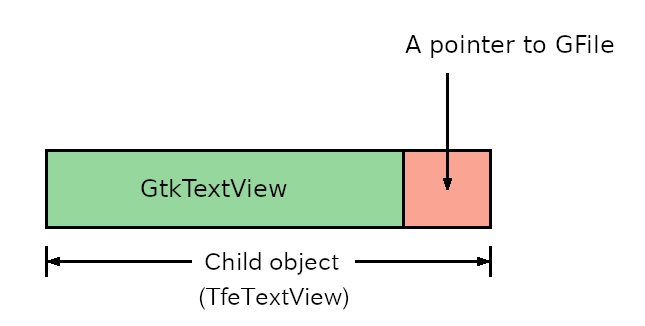
\includegraphics[width=9.675cm,height=4.89cm]{../image/child.png}
\caption{Child object of GtkTextView}
\end{figure}

We will define TfeTextView as a child object of GtkTextView. It has
everything that GtkTextView has. Specifically, TfeTextView has a
GtkTextbuffer which corresponds to the GtkTextView inside TfeTextView.
The additional important thing is that TfeTextView can also keep an
additional pointer to GFile.

In general, this is how GObjects work. Understanding the general theory
about Gobject's is difficult, particularly for beginners. So, I will
just show you the way how to write the code and avoid the theoretical
side. If you want to know about GObject system, refer to another
\href{https://github.com/ToshioCP/Gobject-tutorial}{tutorial}.

\hypertarget{how-to-define-a-child-object-of-gtktextview}{%
\subsection{How to Define a Child Object of
GtkTextView}\label{how-to-define-a-child-object-of-gtktextview}}

Let's define the TfeTextView object, which is a child object of
GtkTextView. First, look at the program below.

\begin{lstlisting}[language=C]
#define TFE_TYPE_TEXT_VIEW tfe_text_view_get_type ()
G_DECLARE_FINAL_TYPE (TfeTextView, tfe_text_view, TFE, TEXT_VIEW, GtkTextView)

struct _TfeTextView
{
  GtkTextView parent;
  GFile *file;
};

G_DEFINE_TYPE (TfeTextView, tfe_text_view, GTK_TYPE_TEXT_VIEW);

static void
tfe_text_view_init (TfeTextView *tv) {
}

static void
tfe_text_view_class_init (TfeTextViewClass *class) {
}

void
tfe_text_view_set_file (TfeTextView *tv, GFile *f) {
  tv -> file = f;
}

GFile *
tfe_text_view_get_file (TfeTextView *tv) {
  return tv -> file;
}

GtkWidget *
tfe_text_view_new (void) {
  return GTK_WIDGET (g_object_new (TFE_TYPE_TEXT_VIEW, NULL));
}
\end{lstlisting}

If you are curious about the background theory of this program, that's
good, because knowing the theory is very important if you want to
program GTK applications. Look at
\href{https://docs.gtk.org/gobject/}{GObject API Reference}. All you
need is described there, or refer to
\href{https://github.com/ToshioCP/Gobject-tutorial}{GObject tutorial}.
It's a tough journey especially for beginners so for now, you don't need
to know about this difficult theory. It is enough to just remember the
instructions below.

\begin{itemize}
\tightlist
\item
  TfeTextView is divided into two parts. Tfe and TextView. Tfe is called
  the prefix, namespace or module. TextView is called the object.
\item
  There are three differnet identifier patterns. TfeTextView (camel
  case), tfe\_text\_view (this is used to write functions) and
  TFE\_TEXT\_VIEW (This is used to cast a pointer to point TfeTextView
  type).
\item
  First, define TFE\_TYPE\_TEXT\_VIEW macro as
  tfe\_text\_view\_get\_type (). The name is always
  (prefix)\_TYPE\_(object) and the letters are upper case. And the
  replacement text is always (prefix)\_(object)\_get\_type () and the
  letters are lower case.
\item
  Next, use G\_DECLARE\_FINAL\_TYPE macro. The arguments are the child
  object name in camel case, lower case with underscore, prefix (upper
  case), object (upper case with underscore) and parent object name
  (camel case).
\item
  Declare the structure \_TfeTextView. The underscore is necessary. The
  first member is the parent object. Notice this is not a pointer but
  the object itself. The second member and after are members of the
  child object. TfeTextView structure has a pointer to a GFile instance
  as a member.
\item
  Use G\_DEFINE\_TYPE macro. The arguments are the child object name in
  camel case, lower case with underscore and parent object type
  (prefix)\_TYPE\_(module).
\item
  Define instance init function (tfe\_text\_view\_init). Usually you
  don't need to do anything.
\item
  Define class init function (tfe\_text\_view\_class\_init). You don't
  need to do anything in this object.
\item
  Write function codes you want to add (tfe\_text\_view\_set\_file and
  tfe\_text\_view\_get\_file). \passthrough{\lstinline!tv!} is a pointer
  to the TfeTextView object instance which is a C-structure declared
  with the tag \_TfeTextView. So, the structure has a member
  \passthrough{\lstinline!file!} as a pointer to a GFile instance.
  \passthrough{\lstinline!tv->file = f!} is an assignment of
  \passthrough{\lstinline!f!} to a member \passthrough{\lstinline!file!}
  of the structure pointed by \passthrough{\lstinline!tv!}. This is an
  example how to use the extended memory in a child widget.
\item
  Write a function to create an instance. Its name is
  (prefix)\_(object)\_new. If the parent object function needs
  parameters, this function also need them. You sometimes might want to
  add some parameters. It's your choice. Use g\_object\_new function to
  create the instance. The arguments are (prefix)\_TYPE\_(object), a
  list to initialize properties and NULL. In this code no property needs
  to be initialized. And the return value is casted to GtkWidget.
\end{itemize}

This program is not perfect. It has some problems. It will be modified
later.

\hypertarget{close-request-signal}{%
\subsection{Close-request signal}\label{close-request-signal}}

Imagine that you are using this editor. First, you run the editor with
arguments. The arguments are filenames. The editor reads the files and
shows the window with the text of files in it. Then you edit the text.
After you finish editing, you exit the editor. The editor updates files
just before the window closes.

GtkWindow emits the ``close-request'' signal before it closes. We
connect the signal and the handler
\passthrough{\lstinline!before\_close!}. A handler is a C function. When
a function is connected to a certain signal, we call it a handler. The
function \passthrough{\lstinline!before\_close!} is invoked when the
signal ``close-request'' is emitted.

\begin{lstlisting}[language=C]
g_signal_connect (win, "close-request", G_CALLBACK (before_close), NULL);
\end{lstlisting}

The argument \passthrough{\lstinline!win!} is a GtkApplicationWindow, in
which the signal ``close-request'' is defined, and
\passthrough{\lstinline!before\_close!} is the handler.
\passthrough{\lstinline!G\_CALLBACK!} cast is necessary for the handler.
The program of \passthrough{\lstinline!before\_close!} is as follows.

\begin{lstlisting}[language=C, numbers=left]
static gboolean
before_close (GtkWindow *win, gpointer user_data) {
  GtkWidget *nb = GTK_WIDGET (user_data);
  GtkWidget *scr;
  GtkWidget *tv;
  GFile *file;
  char *pathname;
  GtkTextBuffer *tb;
  GtkTextIter start_iter;
  GtkTextIter end_iter;
  char *contents;
  unsigned int n;
  unsigned int i;

  n = gtk_notebook_get_n_pages (GTK_NOTEBOOK (nb));
  for (i = 0; i < n; ++i) {
    scr = gtk_notebook_get_nth_page (GTK_NOTEBOOK (nb), i);
    tv = gtk_scrolled_window_get_child (GTK_SCROLLED_WINDOW (scr));
    file = tfe_text_view_get_file (TFE_TEXT_VIEW (tv));
    tb = gtk_text_view_get_buffer (GTK_TEXT_VIEW (tv));
    gtk_text_buffer_get_bounds (tb, &start_iter, &end_iter);
    contents = gtk_text_buffer_get_text (tb, &start_iter, &end_iter, FALSE);
    if (! g_file_replace_contents (file, contents, strlen (contents), NULL, TRUE, G_FILE_CREATE_NONE, NULL, NULL, NULL)) {
      pathname = g_file_get_path (file);
      g_print ("ERROR : Can't save %s.", pathname);
      g_free (pathname);
    }
    g_free (contents);
  }
  return FALSE;
}
\end{lstlisting}

The numbers on the left of items are line numbers in the source code.

\begin{itemize}
\tightlist
\item
  15: Gets the number of pages \passthrough{\lstinline!nb!} has.
\item
  16-29: For loop with regard to the index to each pages.
\item
  17-19: Gets GtkScrolledWindow, TfeTextView and a pointer to GFile. The
  pointer was stored when \passthrough{\lstinline!app\_open!} handler
  had run. It will be shown later.
\item
  20-22: Gets GtkTextBuffer and contents.
  \passthrough{\lstinline!start\_iter!} and
  \passthrough{\lstinline!end\_iter!} are iterators of the buffer. I
  don't want to explain them now because it would take a lot of time.
  Just remember these lines for the present.
\item
  23-27: Writes the contents to the file. If it fails, it outputs an
  error message.
\item
  28: Frees \passthrough{\lstinline!contents!}.
\end{itemize}

\hypertarget{source-code-of-tfe1.c}{%
\subsection{Source code of tfe1.c}\label{source-code-of-tfe1.c}}

The following is the complete source code of
\passthrough{\lstinline!tfe1.c!}.

\begin{lstlisting}[language=C, numbers=left]
#include <gtk/gtk.h>

/* Define TfeTextView Widget which is the child object of GtkTextView */

#define TFE_TYPE_TEXT_VIEW tfe_text_view_get_type ()
G_DECLARE_FINAL_TYPE (TfeTextView, tfe_text_view, TFE, TEXT_VIEW, GtkTextView)

struct _TfeTextView
{
  GtkTextView parent;
  GFile *file;
};

G_DEFINE_TYPE (TfeTextView, tfe_text_view, GTK_TYPE_TEXT_VIEW);

static void
tfe_text_view_init (TfeTextView *tv) {
}

static void
tfe_text_view_class_init (TfeTextViewClass *class) {
}

void
tfe_text_view_set_file (TfeTextView *tv, GFile *f) {
  tv -> file = f;
}

GFile *
tfe_text_view_get_file (TfeTextView *tv) {
  return tv -> file;
}

GtkWidget *
tfe_text_view_new (void) {
  return GTK_WIDGET (g_object_new (TFE_TYPE_TEXT_VIEW, NULL));
}

/* ---------- end of the definition of TfeTextView ---------- */

static gboolean
before_close (GtkWindow *win, gpointer user_data) {
  GtkWidget *nb = GTK_WIDGET (user_data);
  GtkWidget *scr;
  GtkWidget *tv;
  GFile *file;
  char *pathname;
  GtkTextBuffer *tb;
  GtkTextIter start_iter;
  GtkTextIter end_iter;
  char *contents;
  unsigned int n;
  unsigned int i;

  n = gtk_notebook_get_n_pages (GTK_NOTEBOOK (nb));
  for (i = 0; i < n; ++i) {
    scr = gtk_notebook_get_nth_page (GTK_NOTEBOOK (nb), i);
    tv = gtk_scrolled_window_get_child (GTK_SCROLLED_WINDOW (scr));
    file = tfe_text_view_get_file (TFE_TEXT_VIEW (tv));
    tb = gtk_text_view_get_buffer (GTK_TEXT_VIEW (tv));
    gtk_text_buffer_get_bounds (tb, &start_iter, &end_iter);
    contents = gtk_text_buffer_get_text (tb, &start_iter, &end_iter, FALSE);
    if (! g_file_replace_contents (file, contents, strlen (contents), NULL, TRUE, G_FILE_CREATE_NONE, NULL, NULL, NULL)) {
      pathname = g_file_get_path (file);
      g_print ("ERROR : Can't save %s.", pathname);
      g_free (pathname);
    }
    g_free (contents);
  }
  return FALSE;
}

static void
app_activate (GApplication *app, gpointer user_data) {
  g_print ("You need to give filenames as arguments.\n");
}

static void
app_open (GApplication *app, GFile ** files, gint n_files, gchar *hint, gpointer user_data) {
  GtkWidget *win;
  GtkWidget *nb;
  GtkWidget *lab;
  GtkNotebookPage *nbp;
  GtkWidget *scr;
  GtkWidget *tv;
  GtkTextBuffer *tb;
  char *contents;
  gsize length;
  char *filename;
  int i;

  win = gtk_application_window_new (GTK_APPLICATION (app));
  gtk_window_set_title (GTK_WINDOW (win), "file editor");
  gtk_window_maximize (GTK_WINDOW (win));

  nb = gtk_notebook_new ();
  gtk_window_set_child (GTK_WINDOW (win), nb);

  for (i = 0; i < n_files; i++) {
    if (g_file_load_contents (files[i], NULL, &contents, &length, NULL, NULL)) {
      scr = gtk_scrolled_window_new ();
      tv = tfe_text_view_new ();
      tb = gtk_text_view_get_buffer (GTK_TEXT_VIEW (tv));
      gtk_text_view_set_wrap_mode (GTK_TEXT_VIEW (tv), GTK_WRAP_WORD_CHAR);
      gtk_scrolled_window_set_child (GTK_SCROLLED_WINDOW (scr), tv);

      tfe_text_view_set_file (TFE_TEXT_VIEW (tv),  g_file_dup (files[i]));
      gtk_text_buffer_set_text (tb, contents, length);
      g_free (contents);
      filename = g_file_get_basename (files[i]);
      lab = gtk_label_new (filename);
      gtk_notebook_append_page (GTK_NOTEBOOK (nb), scr, lab);
      nbp = gtk_notebook_get_page (GTK_NOTEBOOK (nb), scr);
      g_object_set (nbp, "tab-expand", TRUE, NULL);
      g_free (filename);
    } else if ((filename = g_file_get_path (files[i])) != NULL) {
        g_print ("No such file: %s.\n", filename);
        g_free (filename);
    } else
        g_print ("No valid file is given\n");
  }
  if (gtk_notebook_get_n_pages (GTK_NOTEBOOK (nb)) > 0) {
    g_signal_connect (win, "close-request", G_CALLBACK (before_close), nb);
    gtk_widget_show (win);
  } else
    gtk_window_destroy (GTK_WINDOW (win));
}

int
main (int argc, char **argv) {
  GtkApplication *app;
  int stat;

  app = gtk_application_new ("com.github.ToshioCP.tfe1", G_APPLICATION_HANDLES_OPEN);
  g_signal_connect (app, "activate", G_CALLBACK (app_activate), NULL);
  g_signal_connect (app, "open", G_CALLBACK (app_open), NULL);
  stat =g_application_run (G_APPLICATION (app), argc, argv);
  g_object_unref (app);
  return stat;
}
\end{lstlisting}

\begin{itemize}
\tightlist
\item
  107: Sets the pointer to GFile into TfeTextView.
  \passthrough{\lstinline!files[i]!} is a pointer to GFile structure. It
  will be freed by the system. So you need to copy it.
  \passthrough{\lstinline!g\_file\_dup!} duplicates the given GFile
  structure.
\item
  123: Connects ``close-request'' signal and
  \passthrough{\lstinline!before\_close!} handler. The fourth argument
  is called user data and it is given to the signal handler. So,
  \passthrough{\lstinline!nb!} is given to
  \passthrough{\lstinline!before\_close!} as the second argument.
\end{itemize}

Now compile and run it. There's a sample file in the directory
\passthrough{\lstinline!tfe!}. Type
\passthrough{\lstinline!./a.out taketori.txt!}. Modify the contents and
close the window. Make sure that the file is modified.

Now we got a very simple editor. It's not smart. We need more features
like open, save, saveas, change font and so on. We will add them in the
next section and after.
